%% Complete Article for JIKI Journal
%% Based on Fauzan Husain's research on thermodynamic properties of magnetic models
%% Using Monte Carlo simulations with vertex-cubic spin model

\documentclass[conference, compsoc, twoside]{IEEEtran}

% Essential packages
\usepackage[numbers,sort&compress]{natbib}
\usepackage[labelsep=period,labelfont=bf,justification=justified,font=small]{caption}
\usepackage{balance}
\usepackage{graphicx}
\usepackage{amsmath}
\usepackage{array}
\usepackage[english]{babel}
\usepackage{url}
\usepackage{listings}
\usepackage{inconsolata}
\usepackage[bottom]{footmisc}
\usepackage[top=3cm,bottom=3cm,left=3cm,right=3cm]{geometry}
\usepackage{fancyhdr}
\usepackage{hyperref}

% Code listing setup
\lstset{
  basicstyle=\ttfamily,
}
\captionsetup[lstlisting]{font={small}, labelfont={bf}}

% Header setup
\setlength{\headheight}{22pt}
\pagestyle{fancy}
\fancyhf{}
\setcounter{page}{1}


\renewcommand{\headrulewidth}{0pt}
\fancyhead[LE]{\thepage \textbf{\space \textit{Jurnal Ilmu Komputer dan Informasi (Journal of Computer Science and Information),}} \textit{volume 15,} \\ \textit{ \textrm{ } issue 1, February 2022}}
\fancyhead[LO]{\textit{Fauzan Husain et.al., Thermodynamic Properties of Magnetic Models}}
\fancyhead[RO]{\thepage}

% URL line breaks
\renewcommand{\UrlBreaks}{\do\-}

% Figure and table setup
\def\figurename{Fig.}%
\def\tablename{Table}%

% Path to pictures
\graphicspath{{../pics/}}

\begin{document}

\title{Thermodynamic Properties of Magnetic Models Using Monte Carlo Simulations: A Study of Vertex-Cubic Spin Systems}

\author{\IEEEauthorblockN{Fauzan Husain, Tasrief Surungan\\\\}
	\IEEEauthorblockA{
		\normalfont Department of Physics, Faculty of Mathematics and Natural Sciences, Hasanuddin University, Makassar, Indonesia\\\\
		\textit{Email: fauzanhusain17@gmail.com, tasrief@gmail.com} 
	} \\
}

\twocolumn[
{\csname @twocolumnfalse\endcsname \maketitle}
{\csname @twocolumnfalse\endcsname 
	\renewcommand{\abstractname}{Abstract}
	\begin{abstract}
		\noindent
		\normalfont 
		This research investigates the thermodynamic properties of magnetic models using Monte Carlo simulations with vertex-cubic spin systems. The study focuses on analyzing phase transitions, magnetization behavior, and critical temperature estimation in layered lattice structures. Using the Wolff algorithm for spin updates, we simulate systems with varying lattice sizes (8×8 to 32×32) and layer configurations (1-3 layers). Results show that increasing lattice size sharpens phase transition characteristics, while additional layers shift critical temperatures to higher values and enhance magnetic order stability. The vertex-cubic spin model effectively captures collective behavior in quasi-three-dimensional systems, providing insights into magnetic material properties and phase transition phenomena.
		\\\\
		\noindent
		\textbf{Keywords}: \textit{magnetic models, Monte Carlo simulation, phase transitions, vertex-cubic spin, thermodynamic properties} \\\\
	\end{abstract}
	
	\renewcommand{\abstractname}{Abstrak}
	\begin{abstract}
		\noindent
		\normalfont 
		Penelitian ini menyelidiki sifat-sifat termodinamika model magnetik menggunakan simulasi Monte Carlo dengan sistem spin vertex-kubik. Studi ini berfokus pada analisis transisi fasa, perilaku magnetisasi, dan estimasi suhu kritis dalam struktur kisi berlapis. Menggunakan algoritma Wolff untuk pembaruan spin, kami mensimulasikan sistem dengan ukuran kisi bervariasi (8×8 hingga 32×32) dan konfigurasi lapisan (1-3 lapisan). Hasil menunjukkan bahwa peningkatan ukuran kisi mempertegas karakteristik transisi fasa, sementara penambahan lapisan menggeser suhu kritis ke nilai yang lebih tinggi dan meningkatkan stabilitas orde magnetik. Model spin vertex-kubik secara efektif menangkap perilaku kolektif dalam sistem kuasi-tiga dimensi, memberikan wawasan tentang sifat material magnetik dan fenomena transisi fasa.
		\\\\
		\noindent
		\textbf{Kata Kunci}: \textit{model magnetik, simulasi Monte Carlo, transisi fasa, spin vertex-kubik, sifat termodinamika} \\\\
	\end{abstract}
}
]

\IEEEpeerreviewmaketitle
\thispagestyle{firststyle}

\section{Introduction}

Thermodynamics developed rapidly in the mid-19th century through contributions from figures such as Carnot, Joule, Clausius, and Kelvin, who built the theoretical framework for explaining the macroscopic behavior of physical systems. Statistical mechanics, founded by Boltzmann, connected molecular dynamics with entropy, explaining both macroscopic order and spontaneous fluctuations that occur naturally in physical systems \cite{Pathria2001}.

Research on thermodynamic properties of magnetic materials has been central to condensed matter physics for decades due to both the richness of physical phenomena and potential technological applications. Understanding how microscopic spin interactions influence macroscopic behavior under temperature or magnetic field changes is this study's primary goal. Fig.~\ref{fig:magnetic_classification} shows the classification of magnetic materials based on their response to external magnetic fields.

\begin{figure}[t]
    \centering
    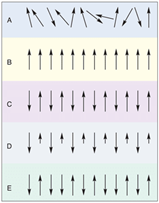
\includegraphics[width=0.9\columnwidth]{Gambar 1. Klasifikasi Magnetik.png}
    \caption{Classification of magnetic materials based on their response to external magnetic fields.}
    \label{fig:magnetic_classification}
\end{figure}

Phase transitions represent one of statistical physics' most fascinating aspects, where changes in macroscopic parameters can trigger drastic changes in a system's collective structure and properties. Studies of phase transitions reveal fundamental material properties and provide insights into system behavior near critical points \cite{Tokura2019}. Fig.~\ref{fig:magnetic_phase_transition} illustrates typical magnetic phase transitions.

\begin{figure}[t]
    \centering
    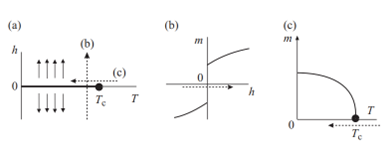
\includegraphics[width=0.9\columnwidth]{Gambar 4. Perubahan Fase Magnetik.png}
    \caption{Magnetic phase transitions showing the change in magnetization as a function of temperature.}
    \label{fig:magnetic_phase_transition}
\end{figure}

Phase transitions relate to system symmetry breaking. For thermally-induced changes, systems exhibit high symmetry at high temperatures as all configuration spaces are accessible. Decreasing temperature reduces thermal fluctuations, leading to stable properties \cite{Surungan2017}.

Spontaneous magnetization is a key phenomenon in phase changes. In ferromagnetic systems, when temperature drops below a critical value (Curie temperature), spontaneous magnetization occurs as the system transitions from paramagnetic to ferromagnetic. This phenomenon is particularly interesting as it involves microscopic spin interactions.

Ernest Ising (1925) introduced a model explaining spontaneous magnetization in ferromagnetic systems. The Ising model, a simplified form of the Heisenberg model, contains discrete variables representing atomic spin magnetic moments with values $s = \pm 1$, interacting with nearest neighbors on a lattice. Fig.~\ref{fig:ising_model} shows the spin orientations in the Ising model.

\begin{figure}[t]
    \centering
    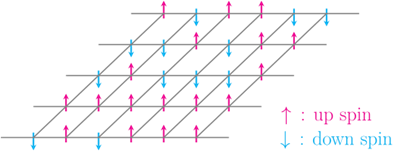
\includegraphics[width=0.9\columnwidth]{Gambar 5. Spin pada Model Ising.png}
    \caption{Spin orientations in the Ising model, showing the discrete nature of spin variables.}
    \label{fig:ising_model}
\end{figure}

The 2D Ising model demonstrates spontaneous magnetization in simple systems. Our study examines the cubic spin model, a discrete spin model with polyhedral symmetry. Polyhedral symmetry for spin models is obtained by dividing the 4$\pi$ solid angle equally from the sphere structure. Five possible model types exist from polyhedral structures: tetrahedron, octahedron, hexahedron, icosahedron, and dodecahedron, as shown in Fig.~\ref{fig:platonic_solids}.

\begin{figure}[t]
    \centering
    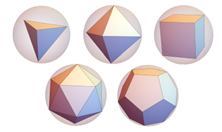
\includegraphics[width=0.9\columnwidth]{Gambar 6. The Platonic Solids.png}
    \caption{The Platonic solids representing the geometric basis for polyhedral spin models.}
    \label{fig:platonic_solids}
\end{figure}

These spins interact like the Ising model. Using Monte Carlo simulation, we can calculate order parameters and estimate critical temperatures. This research focuses on the vertex-cubic spin model, with vertices numbered as shown in Fig.~\ref{fig:cube_vertices}.

\begin{figure}[t]
    \centering
    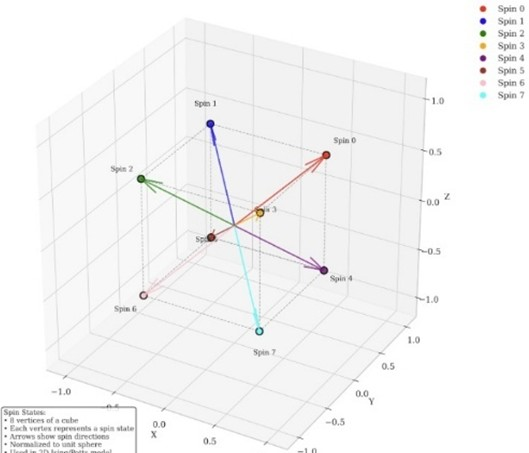
\includegraphics[width=0.9\columnwidth]{Gambar 7. Penommoran Titik Sudut pada Kubus.jpg}
    \caption{Vertex numbering on a cube, illustrating the eight possible spin orientations in the vertex-cubic model.}
    \label{fig:cube_vertices}
\end{figure}

Previous research \cite{Surungan2008} studied ferromagnetic systems on 2D lattices, while other studies \cite{Sutiono2013} examined layered lattice structures (3D). Systems with larger spatial dimensions theoretically have higher critical temperatures due to increased neighbor interactions. Fig.~\ref{fig:layered_lattice} illustrates the layered square lattices used in our simulations.

\begin{figure}[t]
    \centering
    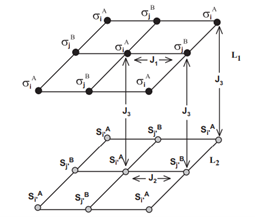
\includegraphics[width=0.9\columnwidth]{Gambar 8. Ilustrasi Kisi Persegi Berlapis.png}
    \caption{Illustration of layered square lattices, showing the structure used in the simulations.}
    \label{fig:layered_lattice}
\end{figure}

This research specifically focuses on studying thermodynamic properties of magnetic models with vertex-cubic spin models on lattices of size $L \times L \times n$. Spin interactions are defined through scalar products of spin vectors, similar to the Heisenberg model discretized on 8 vertex-cubic orientations. We investigate how phase transitions, magnetization, and thermodynamic properties like specific heat are influenced by lattice topology.

\section{Methodology}

\subsection{Vertex-Cubic Spin Model}

The cubic model belongs to polyhedral symmetry with 8 vertices, 6 faces, and 12 edges. The cubic spin model represents spin orientations in three-dimensional space, where spin directions can only point to one of the eight cube vertices. The symmetry follows the $O_h$ group (cubic symmetry group), including rotations and reflections.

This model simplifies the Heisenberg model in discrete form, where spin orientations are limited to eight fixed directions. The distribution of points on the unit sphere surface is quite uniform and symmetric, making this model suitable for describing systems with cubic anisotropy and analyzing magnetic systems with cubic space symmetry.

The cubic spin model is relevant for studying phase transitions and critical properties of three-dimensional systems, especially when continuous approaches are too complex. Despite lower symmetry compared to some other models, its computational simplicity still captures important aspects of collective spin behavior in discrete systems.

\subsection{System Hamiltonian}

The total system energy (Hamiltonian) is defined by interactions between nearest neighbor spins:

\begin{equation}
H = -J \sum_{\langle i,j \rangle} \vec{s_i} \cdot \vec{s_j}
\label{eq:hamiltonian}
\end{equation}

where $J$ is the coupling constant, $\vec{s_i}$ and $\vec{s_j}$ are unit vectors representing spin orientations at sites $i$ and $j$, and the summation $\langle i,j \rangle$ is performed over all nearest neighbor spin pairs \cite{Yunita2022}. In our simulation, $J$ is positive (ferromagnetic) and set to 1 to simplify calculations.

\subsection{Layered Lattice Model}

The layered lattice model extends two-dimensional systems into quasi-three-dimensional systems by adding layers parallel in the third direction. Each layer is a two-dimensional square lattice, connected vertically through interlayer interactions.

This approach allows studying the influence of system thickness on thermodynamic behavior, particularly phase transitions and critical phenomena. Layered lattices help understand the relationship between two-dimensional and three-dimensional systems.

Two-dimensional systems (like the classical Ising model) don't show first-order transitions in certain temperature ranges without domains, while three-dimensional systems facilitate more sudden transitions. Layered structures increase dimensionality, allowing for more robust phase transitions, although each layer experiences two-dimensional dynamics independently.

Studies using effective field theory, Monte Carlo simulation, and renormalization approaches have shown that the number of layers directly affects critical temperature $T_c$ and energy fluctuation intensity. For instance, \cite{Ertaş2014} found that two-layer systems show sharper phase transitions than single-layer systems, and maximum heat capacity values shift to higher temperatures as layers increase.

Layered lattice models also describe real structures such as thin magnetic films, layered two-dimensional materials like graphene, and heterostructures in quantum systems. Interlayer interactions are crucial for understanding phenomena like magnetic anisotropy and spin fields.

\subsection{Finite Size Scaling}

Experiments on real systems and calculations such as Monte Carlo simulations use finite systems. By observing how quantities like specific heat ($C$), magnetization ($M$), and susceptibility ($\chi$) vary with lattice size, we can calculate critical exponent values \cite{Cardy1996}.

Thermodynamic functions are generally extensive quantities, depending on system size. This property allows determination of critical temperature and exponents through Finite Size Scaling. For a thermodynamic function $f(L)$ depending on system size $L$:

\begin{equation}
f(L) = L^g(L)
\label{eq:scaling}
\end{equation}

For systems experiencing second-order phase transitions, $f(L)$ is homogeneous exactly at the critical temperature, meaning $f(L_1) = f(L_2)$ for different system sizes $L_1$ and $L_2$.

For correlation comparison, the scaling function is:

\begin{equation}
Q = f((T - T_c)L^\nu)
\label{eq:correlation}
\end{equation}

where $T$ is system temperature, $T_c$ is the critical temperature, $L$ is the characteristic system size, and $\nu$ is the critical exponent regulating how correlation length diverges near $T_c$. The universal scaling function $f$ implies that data from various system sizes and temperatures will "collapse" into one curve when plotted against $(T - T_c)L^\nu$.

\subsection{Computational Approach}

We used a specialized C program to simulate the thermodynamic properties of cubic magnetic models on quasi-three-dimensional lattices. The program was configured for lattices of size 8×8, 16×16, 24×24, and 32×32 to analyze the effect of system size on results.

The program simulates magnetic systems with cubic-shaped spins (8 possible orientations) on layered two-dimensional lattices with periodic boundary conditions. It calculates thermodynamic parameters such as energy, specific heat, and order parameters at various temperatures to understand phase transitions and critical properties.

\subsubsection{Key Components}

The main components of the simulation include:

\begin{enumerate}
\item \textbf{Initialization}: Setting up simulation parameters, lattice structure, and initial spin configurations.
\item \textbf{Periodic Boundary Conditions}: Ensuring spins at lattice edges interact with opposite sides, simulating infinite systems.
\item \textbf{Spin Orientation Definition}: Defining 8 possible spin orientations representing cubic symmetry.
\item \textbf{Energy Calculation}: Computing interaction energy between spins as $E_{ij} = -(\vec{m_i} \cdot \vec{m_j})$.
\item \textbf{Monte Carlo Steps}: Running equilibration steps followed by measurement steps.
\item \textbf{Wolff Cluster Algorithm}: Implementing efficient spin updates to overcome critical slowing down near phase transitions.
\end{enumerate}

\subsubsection{Measured Parameters}

During simulation, we collected data to calculate:

\begin{enumerate}
\item \textbf{Temperature ($T$)}: Independent variable changed during simulation.
\item \textbf{Quadratic Order Parameter $\langle M^2 \rangle$}: Measures average square of total system magnetization.
\item \textbf{Specific Heat ($C_v$)}: Measures energy fluctuations, calculated from energy variance.
\item \textbf{Binder Cumulant ($U_L$)}: Dimensionless quantity that helps identify phase transitions.
\item \textbf{Internal Energy ($E$)}: Total system energy, reflecting spin order.
\end{enumerate} 

\section{Results and Analysis}

\subsection{Comparison of Observables Between Lattice Sizes}

We analyzed the influence of lattice size $L$ on system behavior for each number of layers. Three main observables were compared: specific heat $C_v$, internal energy $\langle E \rangle$, and magnetic moment ratio $U_L$.

\subsubsection{Specific Heat ($C_v$)}

Specific heat curves display peaks that become higher and sharper as the lattice size increases, characteristic of second-order phase transitions.

For single-layer systems, the $C_v$ peak occurs around temperature $T \approx 0.88$ for $L = 24$, with a relatively large width. The increase in $C_v$ with $L$ appears non-monotonic, likely due to statistical fluctuations or finite-size effects. Fig.~\ref{fig:cv_single_layer} shows the specific heat curve for a single-layer lattice.

\begin{figure}[t]
    \centering
    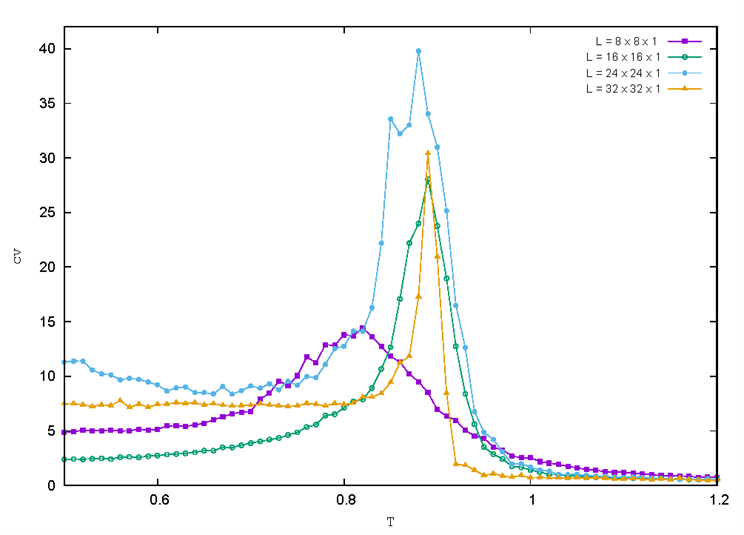
\includegraphics[width=0.9\columnwidth]{Gambar 9. Cv vs T pada Kisi Satu Lapis.png}
    \caption{Specific heat vs. temperature for a single-layer lattice, showing the peak that indicates a phase transition.}
    \label{fig:cv_single_layer}
\end{figure}

For two-layer systems, the specific heat peak shifts to higher temperatures ($T \approx 1.12$) with a more consistent increase in maximum value with $L$. The peak shape becomes sharper, indicating that adding layers increases energy fluctuation strength, as shown in Fig.~\ref{fig:cv_two_layer}.

\begin{figure}[t]
    \centering
    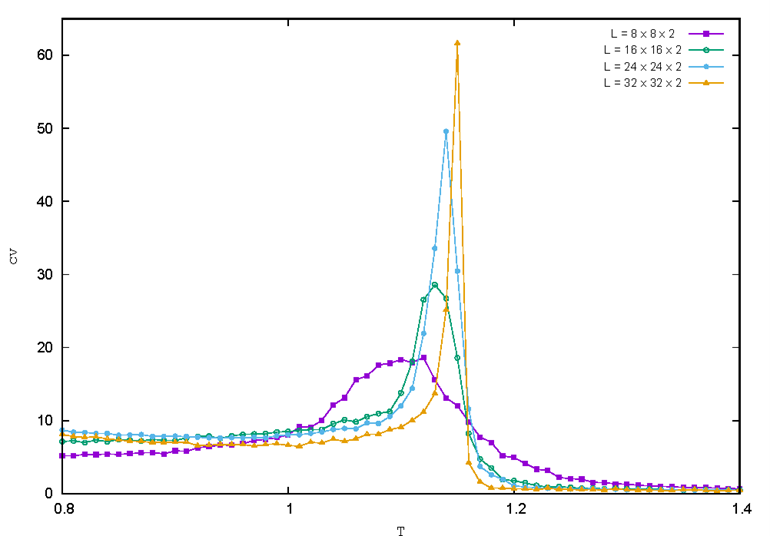
\includegraphics[width=0.9\columnwidth]{Gambar 10. Cv vs T pada Kisi 2 Lapis.png}
    \caption{Specific heat vs. temperature for a two-layer lattice, showing a sharper peak at a higher temperature.}
    \label{fig:cv_two_layer}
\end{figure}

Three-layer systems exhibit the most prominent characteristics. The $C_v$ peak at $L = 32$ reaches values over 90 at temperatures around $T \approx 1.25$, much higher than one or two-layer systems. The sharp increase in maximum values and significant critical temperature shifts indicate that interlayer coupling strengthens spin correlations and clarifies critical phenomena, as demonstrated in Fig.~\ref{fig:cv_three_layer}.

\begin{figure}[t]
    \centering
    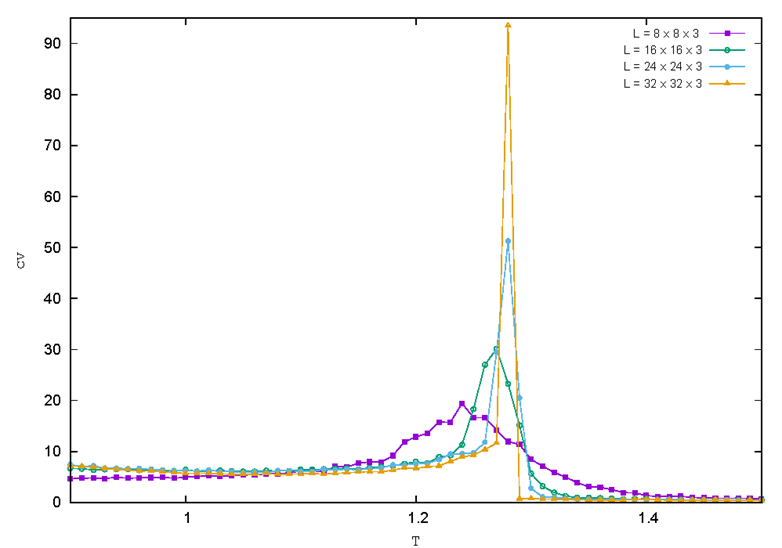
\includegraphics[width=0.9\columnwidth]{Gambar 11. Cv vs T pada Kisi 3 Lapis.png}
    \caption{Specific heat vs. temperature for a three-layer lattice, showing an even sharper peak at a higher temperature.}
    \label{fig:cv_three_layer}
\end{figure}

In general, two main trends emerge: 
\begin{enumerate}
\item Increasing lattice size $L$ produces higher $C_v$ peak values, consistent with finite-size scaling theory for second-order phase transitions.
\item Adding layers $n$ shifts critical temperature toward higher values and produces sharper $C_v$ peaks, indicating that the system approaches three-dimensional behavior.
\end{enumerate}

For the largest lattice size studied (32×32), the specific heat behavior is shown in Fig.~\ref{fig:cv_32x32}.

\begin{figure}[t]
    \centering
    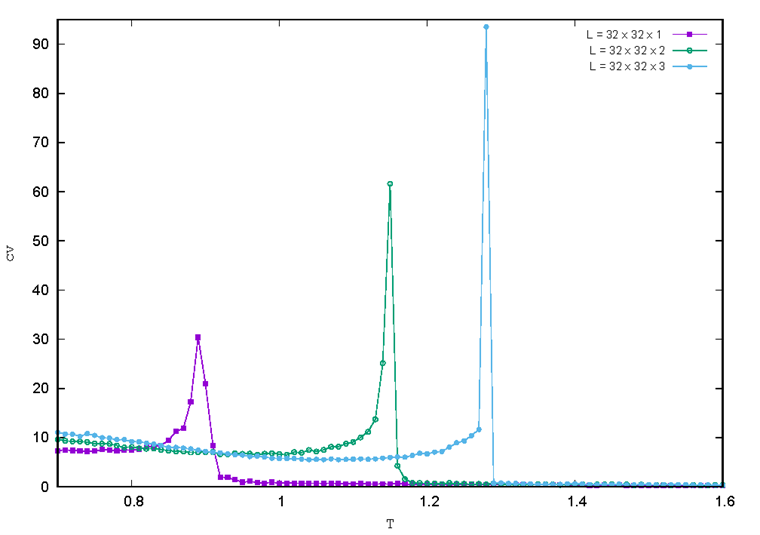
\includegraphics[width=0.9\columnwidth]{Gambar 21. Cv vs T pada Kisi 32 x 32.png}
    \caption{Specific heat vs. temperature for a 32×32 lattice, showing the effect of system size on phase transition characteristics.}
    \label{fig:cv_32x32}
\end{figure}

\subsubsection{Internal Energy $\langle E \rangle$}

Internal energy increases monotonically with temperature, from minimum values at low temperatures toward zero at high temperatures, consistent with spin order decay due to thermal excitation. Fig.~\ref{fig:e_32x32} illustrates this behavior for a 32×32 lattice.

\begin{figure}[t]
    \centering
    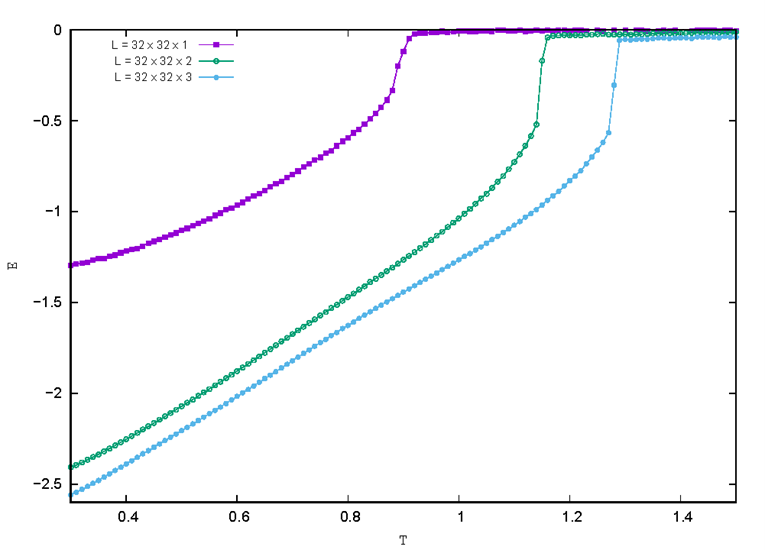
\includegraphics[width=0.9\columnwidth]{Gambar 29. E vs T pada Kisi 32x32.png}
    \caption{Energy vs. temperature for a 32×32 lattice, showing the increase in internal energy with temperature.}
    \label{fig:e_32x32}
\end{figure}

For single-layer systems, energy transitions occur more gradually. For $L = 8$, the energy curve appears smoother due to weaker fluctuations in small systems. At $L = 24$, the energy change gradient is steeper around $T \approx 0.9$, near the phase transition location.

For two-layer systems, minimum energy values decrease compared to single-layer systems, indicating that interlayer interactions strengthen spin order at low temperatures. Energy transitions occur more sharply, especially at $L = 24$, showing significant energy configuration reorganization around $T \sim 1.1$.

Three-layer systems show the steepest energy change gradient around $T \approx 1.25$, consistent with the $C_v$ peak location. The sharp gradient in a narrow temperature interval suggests the system approaches thermodynamic limit behavior where energy changes are non-analytic at the critical temperature.

Our findings indicate that:
\begin{enumerate}
\item Minimum internal energy decreases as the number of layers increases, reflecting additional energy contributions from interlayer coupling.
\item The gradient $\partial E/\partial T$ increases with increasing $L$ and $n$, indicating larger energy fluctuations around the transition temperature.
\item The sharpest energy change shifts to higher temperatures with increasing $n$, consistent with the $T_c$ shift observed in specific heat data.
\end{enumerate}

\subsubsection{Magnetic Moment Ratio ($U_L$)}

The magnetic moment ratio, or Binder cumulant ($U_L = \langle M^4 \rangle/\langle M^2 \rangle^2$), serves as a critical indicator for accurately detecting phase transitions. One advantage of $U_L$ is the existence of intersection points between curves for various system sizes $L$ around the critical temperature $T_c$, relatively free from finite-size effects.

For single-layer systems, curves from $L = 8$ to $L = 32$ show consistent intersections around $T \approx 0.89$, occurring in a narrow range with clear gradients, indicating stable phase transition identification even in limited-size systems.

For two-layer systems, curve intersection points move to $T \approx 1.12$ and become sharper, indicating stronger critical fluctuations. The $U_L$ curves become more separated at low and high temperatures, confirming that the difference between ordered and disordered phases is more pronounced.

Three-layer systems show the most prominent behavior. Intersection points occur at $T \approx 1.25$, and the gradient of $U_L$ changes against temperature becomes very high in the critical region. This emphasizes that increasing layers strengthens transition sharpness and reduces finite-size effects.

Additionally, $U_L$ values at high temperatures approach zero, and at low temperatures approach values close to 2/3, in accordance with theoretical expectations for discrete symmetric systems with bimodal magnetization distribution.

\subsection{Average Square Magnetization $\langle M^2 \rangle$}

For all lattice sizes, $\langle M^2 \rangle$ curves decrease with increasing temperature. Single-layer systems show smoother, more gradual decreases with relatively low magnetization decay points. Fig.~\ref{fig:m2_32x32} illustrates this behavior for a 32×32 lattice.

\begin{figure}[t]
    \centering
    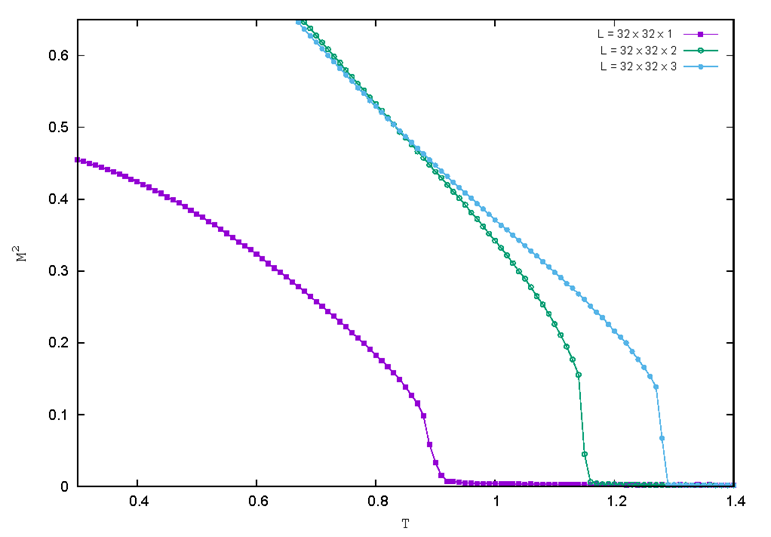
\includegraphics[width=0.9\columnwidth]{Gambar 25. M^2 vs T pada Kisi 32x32.png}
    \caption{Squared magnetization vs. temperature for a 32×32 lattice, showing the decay of magnetic order with increasing temperature.}
    \label{fig:m2_32x32}
\end{figure}

Two-layer and three-layer systems experience sharper decreases at higher temperatures, reflecting increased spin order stability due to interlayer coupling. For $L = 8$, although the curves are relatively smooth, three-layer systems maintain higher $\langle M^2 \rangle$ values at low temperatures and experience slower decay compared to one or two-layer systems.

This pattern becomes more prominent for larger lattices, where transitions from ordered to disordered states appear clearer and steeper, especially in three-layer systems. For $L = 24$ and $L = 32$, $\langle M^2 \rangle$ is almost constant until a certain temperature, then decreases very sharply to zero.

The shift in critical temperature toward higher values for three-layer systems compared to one and two layers shows that system thickness strengthens magnetic stability at higher temperatures, consistent with results from specific heat and magnetic moment ratio.

The behavior of $\langle M^2 \rangle$ also shows the effect of system size: the larger $L$, the steeper the magnetization decrease, indicating that the system begins to represent thermodynamic limit behavior. Phase transitions become increasingly sharp and $\langle M^2 \rangle$ values approach zero simultaneously for all large lattice configurations, consistent with theoretical expectations for discrete spin systems experiencing second-order transitions.

\subsection{Critical Temperature Estimation}

From our analysis, we estimated critical temperatures $T_c$ for various lattice sizes ($L = 8, 16, 24, 32$) and number of layers ($n = 1, 2, 3$). These estimates were obtained from specific heat peaks, sharp changes in internal energy, and decay points of average square magnetization.

The results consistently show that critical temperature increases with both lattice size and number of layers. For single-layer systems, $T_c$ ranges from approximately 0.82 for $L = 8$ to 0.89 for $L = 32$. For two-layer systems, $T_c$ increases to about 1.05 for $L = 8$ and 1.12 for $L = 32$. Three-layer systems show the highest critical temperatures, from approximately 1.18 for $L = 8$ to 1.26 for $L = 32$.

The increase in $T_c$ with layer number reflects the strengthening of spin order due to additional interlayer coupling, making the system more resistant to thermal fluctuations. The variation in $T_c$ with lattice size indicates finite-size effects that gradually diminish as $L$ increases, approaching the thermodynamic limit value.

\section{Conclusion}

Our research on the thermodynamic properties of cubic magnetic models on quasi-three-dimensional lattices has yielded several important findings. Through Monte Carlo simulation with the Wolff algorithm, we observed that:

\begin{enumerate}
\item Increasing lattice size sharpens phase transition characteristics. Specific heat peaks become sharper, magnetization decay becomes clearer, and internal energy changes become steeper, indicating that larger systems more accurately represent thermodynamic behavior.

\item Increasing the number of layers produces more explicit and stable phase transitions. More layers result in higher critical temperatures and stronger spin order until the transition temperature is reached, showing that interlayer coupling plays an important role in strengthening ordered phases.

\item Critical temperatures are identified consistently through specific heat peaks, minimum Binder Cumulant, and magnetization decay. Critical temperature increases with increasing lattice size and number of layers, and is more stable in large systems with multiple layers.

\item The magnetic moment ratio shows that spin order is more stable in layered systems, even at temperatures approaching the transition. Binder Cumulant intersections become sharper with increasing $L$ and $n$, indicating stronger critical behavior.

\item The layered vertex-cubic spin model effectively describes intermediate-dimensional physical systems like thin magnetic films or layered structures. This approach proves effective for studying phase transitions in systems with discrete orientations and limited spatial interactions.
\end{enumerate}

Our results demonstrate that the vertex-cubic spin model accurately captures collective behavior in quasi-three-dimensional systems, providing valuable insights into magnetic material properties and phase transition phenomena. Future research could extend this model to other polyhedral symmetries or investigate the effects of disorder and external fields on critical behavior.

\section*{Acknowledgement}

The authors would like to thank the research community for their valuable contributions to the field of statistical physics and magnetic materials. Special thanks to the reviewers for their constructive feedback.

\balance

\bibliographystyle{IEEEtran}
\bibliography{IEEEabrv,references}

\end{document} 